\documentclass[12pt, a4paper]{article}
\usepackage[a4paper,margin=1in,footskip=0.25in]{geometry}
 
\usepackage{graphicx}
\usepackage{enumerate}
\usepackage{amsmath}
\usepackage{amssymb}
\usepackage[utf8]{inputenc}
\usepackage{physics}
\usepackage{xcolor}
\usepackage{hyperref}
\usepackage{subfig}

\captionsetup[subfigure]{justification=raggedright}

\providecommand{\newoperator}[3]{%
	\newcommand*{#1}{\mathop{#2}#3}}
\providecommand{\renewoperator}[3]{%
	\renewcommand*{#1}{\mathop{#2}#3}}
	
\newoperator{\srot}%
	{\mathrm{rot}}{\nolimits}

\newoperator{\ent}%
	{\mathrm{ent}}{\nolimits}
	
\renewoperator{\Re}%
	{\mathrm{Re}}{\nolimits}
	
\renewoperator{\Im}%
	{\mathrm{Im}}{\nolimits}	
	
\makeatletter
\providecommand*{\diff}%
	{\@ifnextchar^{\DIfF}{\DIfF^{}}}
	
\def\DIfF^#1{%
	\mathop{\mathrm{\mathstrut d}}%
	\nolimits^{#1}\gobblespace}
	
\def\gobblespace{%
	\futurelet\diffarg\opspace}
	
\def\opspace{%
	\let\DiffSpace\!%
		\ifx\diffarg(%
			\let\DiffSpace\relax
		\else
			\ifx\diffarg[%
				\let\DiffSpace\relax
			\else
				\ifx\diffarg\{%
					\let\DiffSpace\relax
				\fi\fi\fi\DiffSpace}
				
\providecommand*{\deriv}[3][]{%
	\frac{\diff^{#1}#2}{\diff #3^{#1}}}
\providecommand*{\pderiv}[3][]{%
	\frac{\partial^{#1}#2}%
		{\partial #3^{#1}}}
		
\newcommand{\mean}[1]{\langle#1\rangle}

\begin{document}

\section{The~Model}
We investigate the~$XXZ$~model in one-dimension (1D) with periodic boundary conditions (PBC),
\begin{equation}
H = J\sum_{\mean{i,j}} \alpha S_i^x S_j^x + S_i^y S_j^y + S_i^z S_j^z,
\end{equation}
where $\alpha \in [0, 1]$. In the limit of $\alpha = 1$ the above resembles exactly the Heisenberg model, while for $\alpha = 0$ it is the isotropic case of the~$XY$~model. Typically one puts the parameter $\alpha$ in front of the $z$~component of the spin operators. However then the $z$~axis is not a good quantization axis in $\alpha \to 0$ limit. Assuming natural alignment of the spin chain along the $x$-axis we decide to scale spin interaction along the chain while keeping the interactions in the perpendicular $YZ$ plane untouched.

In particular we are interested in the~$J < 0$ case for limiting and intermediate values of parameter $\alpha$. The quantity of interest is the spectral function of the single spin excitation with momentum $q$,
\begin{equation}
S(q,\omega) = -\frac{1}{\pi} \lim_{\delta\to 0^+} \Im\bra{\textsc{gs}}S_q^+ G(\omega + i\delta) S_q^- \ket{\textsc{gs}},
\end{equation}
where
\begin{equation}
G(\omega) = \left(\omega - H + E_{\textsc{gs}}\right)^{-1}.
\end{equation}
We aim at identifying and understanding processes leading to change from single magnon branch in the $S(q,\omega)$ for $\alpha = 1$ to the two-spinon continuum in $\alpha = 0$ limit. In particular we would like to find out whether the magnon-magnon interactions play any (important) role in the above mentioned evolution of the spectral function.

\section{Methodology}
Let us firstly rewrite the $XXZ$~Hamiltonian in somewhat more convenient form. We~start by introducing the spin rising and lowering operators,
\begin{equation}
\begin{aligned}
S_i^x = \frac{1}{2}\left(S_i^+ + S_i^-\right), \\
S_i^y = \frac{1}{2i}\left(S_i^+ - S_i^-\right).
\end{aligned}
\end{equation}
With the above on can split the model Hamiltonian into two parts, the Heisenberg Hamiltonian (denoted here as \textit{parallel} $\parallel$) and \textit{rotated} Heisenberg Hamiltonian (denoted as \textit{perpendicular} $\perp$),
\begin{equation}\label{eq:H_parts}
H = \frac{1+\alpha}{2} H_{\parallel} + \frac{1-\alpha}{2} H_{\perp},
\end{equation}
where
\begin{equation}\label{eq:H_parallel}
H_{\parallel} = J\sum_{\mean{i,j}}S_i^z S_j^z + \frac{1}{2}\left(S_i^+ S_j^- + S_i^- S_j^+\right),
\end{equation}
and
\begin{equation}\label{eq:H_perpendicular}
H_{\perp} = J\sum_{\mean{i,j}} S_i^z S_j^z - \frac{1}{2}\left(S_i^+ S_j^+ + S_i^- S_j^-\right).
\end{equation}

\subsection{Clarification of the notation}
Let us comment on why we call $H_{\perp}$ the \textit{rotated} Heisenberg Hamiltonian. Consider a transformation rotating spins at every second site, e.g. on the sublattice $\mathcal{B}$,
\begin{equation}
\srot : \forall j\in\mathcal{B} \ (S_j^{\pm} \rightarrow S_j^{\mp}) \land (S_j^{z} \rightarrow -S_j^{z}).
\end{equation}
The stated-above transformation reveals the relation between $H_{\parallel}$ and $H_{\perp}$, namely,
\begin{equation}\label{eq:rot_relation}
\srot H_{\parallel} = -H_{\perp}.
\end{equation}
Now let us comment on why we denoted these Hamiltonians as \textit{parallel} and \textit{perpendicular} accordingly. There are two reasons. 

The first come from the magnetization conservation present in the Heisenberg model. Indeed, one can see that $S_i^+ S_j^- + S_i^- S_j^+$ operators allow the magnetic excitation (flipped spin) to spread only across states within the subspace of the Hilbert space corresponding to the given magnetization because number of spins up or/and down cannot be changed. On the other hand $S_i^+ S_j^+ + S_i^- S_j^-$ operators come with the opposing mechanism leading to changes in the magnetization of the system. 

The second reason for the choice of the notation comes from the type of the \textit{classical} ground state of the system realised by these models. For ferromagnetic coupling constant $(J < 0)$ the ground state of $H_{\parallel}$ is $2S+1$ degenerated due to rotational symmetry of the system. But in the thermodynamic limit and arbitrary small magnetic field the symmetry is broken and the system appears to be in ferromagnetic state, i.e. neighbouring spins are aligned parallel in the \textit{classical} ground state. Accordingly, for antiferromagnetic coupling constant $(J > 0)$ the Ising antiferromagnet is within possible ground states of $H_{\perp}$ (formally also $2S+1$ degenerated).

\subsection{Magnetization and Staggered Magnetization}
In order to understand how the classical antiferromagnet arises as the ground state of $H_{\perp}$ for $J > 0$ it is enough to look at the Eq.~(\ref{eq:rot_relation}). Rotating the operators in the Heisenberg model and spins in the sublattice $\mathcal{B}$ one does not change the physics of the system. Therefore given the eigenstates $\ket{\psi_n}$ of $H_{\parallel}$ Hamiltonian with corresponding energies $E_n$ one easily obtains eigenstates of the $H_{\perp}$ by reversing spins at sublattice $\mathcal{B}$. Then corresponding energies are $-E_n$. Incorporating the sign change into a coupling constant we see that Ising antiferromagnet is the ground state of $H_{\perp}$ for antiferromagnetic $J > 0$. 

Above-described relation between eigenstates of these two Hamiltonians allow one to make even stronger statement, namely: in order to understand $H_{\perp}$ one just need to consider the Heisenberg model for opposing sign of the coupling constant $J$. Thus, any quantity of $H_{\parallel}$ should have its corresponding \textit{staggered}-quantity in $H_{\perp}$ related by the rotation of $\mathcal{B}$ sublattice. Therefore, for example, if $H_{\parallel}$ Hamiltonian conserves the magnetization,
\begin{equation}
M = \sum_{i = 0,\hdots,N-1} S_i^z,
\end{equation}
then $H_{\perp}$ Hamiltonian conserves the staggered magnetization
\begin{equation}
M_s = \sum_{i = 0,\hdots,N-1} (-1)^i S_i^z.
\end{equation}

\subsection{Interplay of the two parts of the Hamiltonian}
The ground state of the Heisenberg model $H_{\parallel}$ for antiferromagnetic coupling constant is given by a certain linear combination of the $S^z$ spins configurations. It belongs to the subspace where absolute value of the magnetization is smallest possible, i.e. $M = 0$ for even number of spins or $|M| = 1/2$ for odd number of spins. Accordingly the ground state of rotated Heisenberg $H_{\perp}$ for ferromangetic coupling constant is a linear combination of states belonging to the subspace with staggered magnetization $M_s = 0$ (assuming even number of spins). Thus the full model tries to maximize magnetization and minimize staggered magnetization. It is important to notice that this is not the same and the two parts of the Hamiltonian play towards rather orthogonal than totally parallel or antiparallel goal. While pure ferromagenetic Heisenberg model prefers simple ferromagnetic ground state the contribution from rotated Heisenberg will lead to changes in magnetization via double spin flips processes, i.e. $S_i^+ S_j^+ + S_i^- S_j^-$. This will further unlock the $S_i^+ S_j^- + S_i^- S_j^+$ terms leading to the break of the staggered magnetization conservation of the pure rotated Heisenberg. In the end the ground state will be a complicated linear combination of states belonging to various magnetization and staggered magnetization subspaces. Shortly speaking,
\begin{equation}
[H_{\parallel}, H_{\perp}] \neq 0.
\end{equation}

\subsection{Exact diagonalization studies of small systems}
In this subsection we will analise the model for small systems. Let us start with the two site chain including PBC (this just effectively multiplies the coupling constant by a factor of 2 in this case but we would like to preserve the PBC for all the cases). We have four possible states,
\begin{equation}
\ket{0} = \ket{\downarrow\downarrow}, \quad \ket{1} = \ket{\downarrow\uparrow}, \quad \ket{2} = \ket{\uparrow\downarrow}, \quad \ket{3} = \ket{\uparrow\uparrow},
\end{equation}
and therefore in the ordered basis
\begin{equation}
\mathcal{B} = \big(\ket{0}, \ket{1}, \ket{2}, \ket{3}\big),
\end{equation}
where we use the $n$-tuple notation to explicitly denote the sequence of basis vectors. Thus matrix of the model Hamiltonian in basis $\mathcal{B}$ appears as follows,
\begin{equation}
\mathcal{M}(H)_{\mathcal{B}}^{\mathcal{B}} = \frac{J}{2} \begin{pmatrix}
1 & 0 & 0 & -(1-\alpha) \\
0 & -1 & 1+\alpha & 0 \\
0 & 1+\alpha & -1 & 0 \\
-(1-\alpha) & 0 & 0 & 1
\end{pmatrix}.
\end{equation}
We know the model does not conserve magnetization nor staggered magnetization. Nevertheless one still can notice that parity of the magnetization and the parity of staggered magnetization cannot be affected by the model Hamiltonian. This allows us to classify each state to one and only one out of four classes of states. The classes are following,
\begin{itemize}
	\item $S_0 = \{\psi : (M\ket{\psi}\mod 2 = 0) \land  (M_s \ket{\psi}\mod 2 = 0)\}$,
	\item $S_1 = \{\psi : (M\ket{\psi}\mod 2 = 0) \land  (M_s \ket{\psi}\mod 2 = 1)\}$,
	\item $S_2 = \{\psi : (M\ket{\psi}\mod 2 = 1) \land  (M_s \ket{\psi}\mod 2 = 0)\}$,
	\item $S_3 = \{\psi : (M\ket{\psi}\mod 2 = 1) \land  (M_s \ket{\psi}\mod 2 = 1)\}$.
\end{itemize}
For the considered case of two sites let us find out which state belongs to which subspace. We have,
\begin{itemize}
	\item $(M\ket{0} = -1) \land (M_s\ket{0} = 0) \Rightarrow \ket{0} \in S_2$, 
	\item $(M\ket{1} = 0) \land (M_s\ket{1} = 1) \Rightarrow \ket{1} \in S_1$, 
	\item $(M\ket{2} = 0) \land (M_s\ket{2} = -1) \Rightarrow \ket{2} \in S_1$, 
	\item $(M\ket{3} = 1) \land (M_s\ket{3} = 0) \Rightarrow \ket{3} \in S_2$.
\end{itemize}
One can see we could assign these states to two out of four possible subspaces. In general for system with $n = 4k - 2$ lattice sites (where $k \in \mathbb{N}$) all the states can be assigned either to subspace $S_1$ or $S_2$, whereas for $n = 4k$ states belong either to subspace $S_0$ or $S_3$. Now, reordering the ordered basis $\mathcal{B}$,
\begin{equation}
\mathcal{B} \rightarrow \mathcal{B}' = \big(\ket{1}, \ket{2}, \ket{0}, \ket{3}\big),
\end{equation}
we obtain the matrix of the Hamiltonian consisting of two blocks corresponding to the two orthogonal subspaces,
\begin{equation}
\mathcal{M}(H)_{\mathcal{B}'}^{\mathcal{B}'} = \frac{J}{2} \begin{pmatrix}
-1 & 1+\alpha & 0 & 0 \\
1+\alpha & -1 & 0 & 0 \\
0 & 0 & 1 & -(1-\alpha) \\
0 & 0 & -(1-\alpha) & 1
\end{pmatrix}.
\end{equation}
For $\alpha \in [0, 1)$ the above can be easily diagonalized yielding following eigenstates and energies,
\begin{eqnarray}
\ket{\psi_1} &=& \frac{1}{\sqrt{2}}\left(\ket{2} + \ket{1}\right), \quad E_1 = \frac{J}{2}\alpha, \\
\ket{\psi_2} &=& \frac{1}{\sqrt{2}}\left(\ket{2} - \ket{1}\right), \quad E_2 = -\frac{J}{2}(2+\alpha), \\
\ket{\psi_3} &=& \frac{1}{\sqrt{2}}\left(\ket{3} + \ket{0}\right), \quad E_3 = \frac{J}{2}\alpha, \\
\ket{\psi_4} &=& \frac{1}{\sqrt{2}}\left(\ket{3} - \ket{0}\right), \quad E_4 = \frac{J}{2}(2-\alpha).
\end{eqnarray}
For ferromagnetic $J < 0$ the ground state energy is $E_4$. It is also true that for a finite system the ground state is always a singlet (see results in Sec. \ref{sec:ed_results}). This changes at $\alpha = 1$, i.e. in the case of the Heisenberg model, where for ferromagnetic coupling constant one expects a triplet in the two site example. Also note that for $\alpha = 1$ the coupling between $\ket{0}$ and $\ket{3}$ vanish. Thus case of $\alpha = 1$ is qualitatively different and should be investigated separately from the $\alpha \in [0, 1)$. 

Let now have a look at the four sites case. There are 16 possible spin states separable into two subspaces of equal sizes. We can enumerate these states using binary representation for each spin configuration as in the two site example, 
\begin{equation}
\ket{\downarrow\downarrow\downarrow\downarrow} = \ket{0}, \quad \ket{\downarrow\downarrow\downarrow\uparrow} = \ket{1}, \quad ..., \quad \ket{\uparrow\uparrow\uparrow\uparrow} = \ket{15}.
\end{equation}
Thus for the subspace with even magnetization and even staggered magnetization we may choose the following ordered basis,
\begin{equation}
\mathcal{C}_0 = \Big( \ket{0}, \ket{3}, \ket{5}, \ket{6}, \ket{9}, \ket{10}, \ket{12}, \ket{15} \Big),
\end{equation}
whereas for the subspace with odd magnetization and odd staggered magnetization the ordered basis may appear as follows,
\begin{equation}
\mathcal{C}_1 = \Big( \ket{1}, \ket{2}, \ket{4}, \ket{7}, \ket{8}, \ket{11}, \ket{13}, \ket{14} \Big).
\end{equation}
Thus matrix of the Hamiltonian consists of two blocks,
\begin{equation}
\mathcal{M}(H)_{\mathcal{C}_0}^{\mathcal{C}_0} = \frac{J}{2} \begin{pmatrix}
2 & \tau_{\perp} & 0 & \tau_{\perp} & \tau_{\perp} & 0 & \tau_{\perp} & 0 \\
\tau_{\perp} & 0 & \tau_{\parallel} & 0 & 0 & \tau_{\parallel}  & 0 & \tau_{\perp}\\
0 & \tau_{\parallel}  & -2 & \tau_{\parallel} & \tau_{\parallel}  & 0 & \tau_{\parallel}  & 0 \\
\tau_{\perp}& 0 & \tau_{\parallel} & 0 & 0 & \tau_{\parallel}  & 0 & \tau_{\perp} \\
\tau_{\perp}& 0 & \tau_{\parallel} & 0 & 0 & \tau_{\parallel}  & 0 & \tau_{\perp} \\
0 & \tau_{\parallel}  & 0 & \tau_{\parallel} & \tau_{\parallel}  & -2 & \tau_{\parallel}  & 0 \\
\tau_{\perp} & 0 & \tau_{\parallel} & 0 & 0 & \tau_{\parallel}  & 0 & \tau_{\perp}\\
0 & \tau_{\perp} & 0 & \tau_{\perp} & \tau_{\perp} & 0 & \tau_{\perp} & 2
\end{pmatrix},
\end{equation}
\begin{equation}
\mathcal{M}(H)_{\mathcal{C}_1}^{\mathcal{C}_1} = \frac{J}{2} \begin{pmatrix}
0 & \tau_{\parallel} & 0 & \tau_{\perp} & \tau_{\parallel} & 0 & \tau_{\perp} & 0 \\
\tau_{\parallel} & 0 & \tau_{\parallel} & 0 & 0 & \tau_{\perp}  & 0 & \tau_{\perp}\\
0 & \tau_{\parallel}  & 0 & \tau_{\perp} & \tau_{\parallel}  & 0 & \tau_{\perp}  & 0 \\
\tau_{\perp}& 0 & \tau_{\perp} & 0 & 0 & \tau_{\parallel}  & 0 & \tau_{\parallel} \\
\tau_{\parallel}& 0 & \tau_{\parallel} & 0 & 0 & \tau_{\perp}  & 0 & \tau_{\perp} \\
0 & \tau_{\perp}  & 0 & \tau_{\parallel} & \tau_{\perp}  & 0 & \tau_{\parallel}  & 0 \\
\tau_{\perp} & 0 & \tau_{\perp} & 0 & 0 & \tau_{\parallel}  & 0 & \tau_{\parallel}\\
0 & \tau_{\perp} & 0 & \tau_{\parallel} & \tau_{\perp} & 0 & \tau_{\parallel} & 0
\end{pmatrix},
\end{equation}
where
\begin{equation}\label{eq:tau_def}
\tau_{\parallel} = \frac{1+\alpha}{2}, \quad \text{and} \quad \tau_{\perp} = -\frac{1-\alpha}{2}
\end{equation}
Diagonalizing each subspace we obtain set of eigenvectors and energies where the ground state energy is $E_\textsc{gs} = E^\textsc{gs}_{\mathcal{C}_0} = \frac{J}{2}\left(-\alpha + \sqrt{8 + \alpha^2}\right)$. It is also worth of noticing that the second lowest energy in the subspace containing the ground state is equal to the lowest energy in the other one subspace $E^{\textsc{gs}}_{\mathcal{C}_1} = J$. Here $E^{\textsc{gs}}_{\mathcal{C}_1}$ does not depend on $\alpha$ but in general, e.g. for larger systems, it does. Similarly we had $E_1 = E_3 = \frac{J}{2}\alpha$ in the two site example. The same holds for any lattice size $n = 2k$ -- second lowest energy is at least doubly degenerated and corresponding eigenstates belong to different subspaces with respect to parity of magnetization and staggered magnetization. 

Cases with odd number of lattice sites are different with the ground state being doubly degenerated for $\alpha \in [0, 1)$ and we are not going to investigate them in details here. Nevertheless we can draw a conclusion for cases with even number of lattice sites. Namely, when number of lattice sites grows the two lowest energies should approach one another because in the thermodynamic limit one shall not be able to distinguish between even and odd number of lattice sites.

\subsection{Transformation to Bosonic Hamiltonian}
We would like to investigate the role of magnon-magnon interactions in the XXZ~model. Therefore we have to reformulate the model Hamiltonian originally written in fermionic spin operators. The required relations are given by the Holstein-Primakoff transformation for spin $S = 1/2$,
\begin{equation}
	S_i^+ = a_i^\dagger P(n_i), \quad\quad
	S_i^- = P(n_i) a_i, \quad\quad
	S_i^z = n_i - \frac{1}{2},
\end{equation}
where $n_i = a_i^\dagger a_i$ and,
\begin{equation}
	P(n_i) = \sqrt{1 - n_i}.	
\end{equation}
We could expand the function $P(x)$ into a Taylor series. However this approach has a~huge drawback -- one needs infinitely many terms in order to obtain exact representation of $P$. Instead we will use Newton series which is exact at integer values of $x$. Since $n_i$ always takes integer values this approach allows us to represent $P(n_i)$ exactly in a finite (i.e. $2S+1$) number of terms \cite{knig2020newton}, 
\begin{equation}
	s = \frac{1}{2} \Rightarrow P(n_i) = 1 - n_i.
\end{equation}

Applying the Holstein-Primakoff transformation to the Heisenberg (Eq.~\ref{eq:H_parallel}) and rotated Heisenberg (Eq.~\ref{eq:H_perpendicular}) Hamiltonians we obtain,
\begin{eqnarray}
	H_{\parallel} &=& J\sum_{\mean{i,j}} \left(n_i - \frac{1}{2}\right) \left(n_j - \frac{1}{2}\right) + \frac{1}{2}\left(a_i^\dagger P(n_i) P(n_j) a_j + P(n_i) a_i a_j^\dagger P(n_j)\right), \\
	H_{\perp} &=& J\sum_{\mean{i,j}} \left(n_i - \frac{1}{2}\right) \left(n_j - \frac{1}{2}\right) - \frac{1}{2}\left(a_i^\dagger P(n_i) a_j^\dagger P(n_j) + P(n_i) a_i P(n_j) a_j\right).
\end{eqnarray}
Following the Eqs.~\ref{eq:H_parts}~and~\ref{eq:tau_def}, we arrive at the model Hamiltonian expressed through bosonic operators,
\begin{eqnarray}\label{eq:H_bosonic}
	H &=& H_{\mathcal{T}} + H_{\mathcal{V}}, \\
	H_{\mathcal{V}} &=& J\sum_{\mean{i,j}} \frac{1}{4} - \frac{1}{2}\left(n_i + n_j\right) + \beta n_i n_j, \\
	H_{\mathcal{T}} &=& \frac{J\tau_{\parallel}}{2} \sum_{\mean{i,j}} a_i^\dagger (1-n_i)(1-n_j)a_j + \frac{\tau_{\perp}}{\tau_{\parallel}} a_i^\dagger a_j^\dagger (1-n_i) (1-n_j) + \text{H.c.}
\end{eqnarray}
where the perameter $\beta = 1$ indicates the exact transformations with magnon-magnon interactions taken into account. Putting $\beta = 0$ switch the interactions off. Investigating the model in both limits of parameter $\beta$ we hope to understand the role of magnon-magnon interactions. Note that $1-n_i$ terms ensure we have at most one magnon at single site. Since their role is merely a projection onto a proper subspace we do not consider them as part of magnon-magnon interactions. From the above-defined transformation it follows that previously defined state $\ket{\downarrow\downarrow\downarrow\downarrow} = \ket{0} = \ket{0 0 0 0}$ does not have magnons while the state $\ket{\uparrow\uparrow\uparrow\uparrow} = \ket{15} = \ket{1 1 1 1}$ is fully occupied by magnons.

\section{Exact Diagonalisation Results}\label{sec:ed_results}
In what follows we investigate larger systems in the range of parameter $\alpha \in [0, 1)$ and magnon-magnon interactions both present ($\beta = 1$) or absent ($\beta = 0$). In addition we look also at intermadiate values of $\beta$ and the limit of $\beta \to -\infty$ in order to understand the role of magnon-magnon interactions.

\subsection{XY~Model Limit}\label{sec:XY_model}
Let us start with $\alpha = 0$ limit of the XXZ~model, the XY~model. In this limit the model can be solved exactly. The XY~model can be understood as a theory of free spinless fermions with nearest neighbour hopping. In order to arrive at this result one introduces rising and lowering operators and proceeds with Jordan-Wigner transformation \cite{JordanWigner}. The~spectral function of the~XY~model obtained using exact diagonalization (ED) is~presented in~the~Figure~\ref{fig:XY_int}.
\begin{figure}[ht]
	\centering
	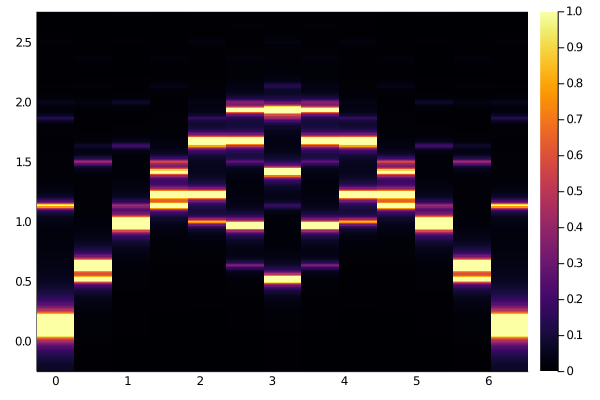
\includegraphics[width=0.75\textwidth]{../figures/fig001.png}
	\caption{Spectral function $S(q,\omega)$ of a single spin flip (magnon excitation) for $\alpha = 0$ and $\beta = 1$ limit of XXZ~model (i.e. XY~model limit).}\label{fig:XY_int}
\end{figure}

Let see how the spectrum changes when we turn the magnon-magnon interactions off ($\beta = 0$). The~results are presented in the Figure~\ref{fig:XY_noint}. The spectral function looks similar to single magnon in the case of the ferromagnetic Heisenberg model. In fact it is something in between but visibly it bears more resemblence to the single branch than the continuum. In order to understand how does a single branch appears as a solution it is instructive to investigate limit of $\beta \to -\infty$. The spectral function in this case is presented in the Figure~\ref{fig:XY_limit}. 

In the limit of $\beta \to -\infty$ it is basically not possible to have states with two neighbouring magnons, see Eq.~(\ref{eq:H_bosonic}) due to infinite energy cost (for ferromagnetic $J<0$). Therefore terms proportional to $\tau_{\perp}$ in Eq.~(\ref{eq:H_bosonic}) effectively do not play a role. In spin language this means that terms $S_i^+ S_j^+$ and $S_i^- S_j^-$ that are present in the model for $\alpha < 1$ (see Eq.~(\ref{eq:H_perpendicular})) are suppressed. The ground state of the system is the state without magnons, i.e. the state with all the spins pointing down in our case (i.e a particular N\'eel state). Thus it is not suprissing why the spectral function of a single spin flip looks like in the case of the ferromagnetic Heisenberg model. Nevertheless, it is still interresting that switching the interactions off ($\beta = 1 \rightarrow \beta = 0$) influences the spectrum in such a drastic way while difference between spectral function for $\beta = 0$ and $\beta \to -\infty$ is barely visible.
\begin{figure}[ht]
	\centering
	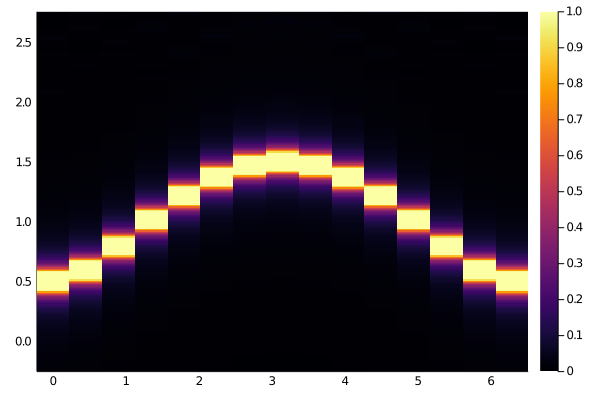
\includegraphics[width=0.75\textwidth]{../figures/fig002.png}
	\caption{Spectral function $S(q,\omega)$ of a single spin flip (magnon excitation) for $\alpha = 0$ and $\beta = 0$ limit of XXZ~model (i.e. XY~model limit).}\label{fig:XY_noint}
\end{figure}
\begin{figure}[h!]
	\centering
	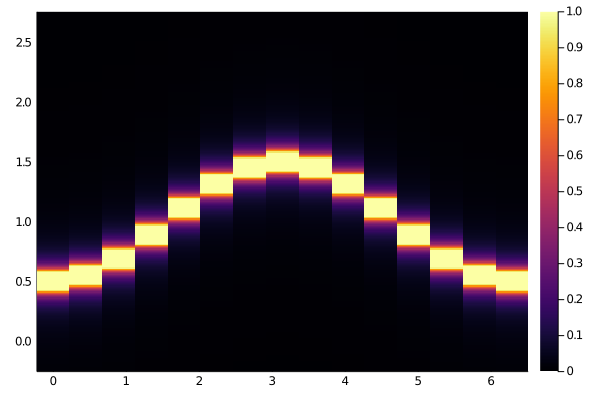
\includegraphics[width=0.75\textwidth]{../figures/fig003.png}
	\caption{Spectral function $S(q,\omega)$ of a single spin flip (magnon excitation) for $\alpha = 0$ and $\beta \to -\infty$ limit of XXZ~model (i.e. XY~model limit).}\label{fig:XY_limit}
\end{figure}

Let us now investigate how the spectrum evolves when we change the \textit{strength} of magnon-magnon interactions, i.e. when we contunuously change the parameter $\beta \in [0,1]$. Figure~\ref{fig:XY_beta_dep} shows calculated results for varius $\beta$ values.
\begin{figure}
	\centering
	\subfloat[$\beta = 1.0$]{
		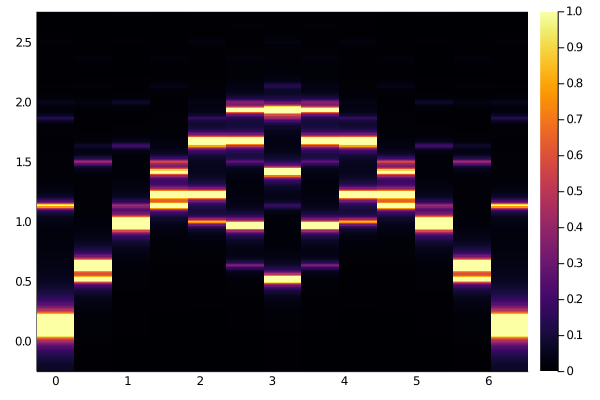
\includegraphics[width=0.45\textwidth]{../figures/fig001.png}
	}
	\subfloat[$\beta = 0.95$]{
		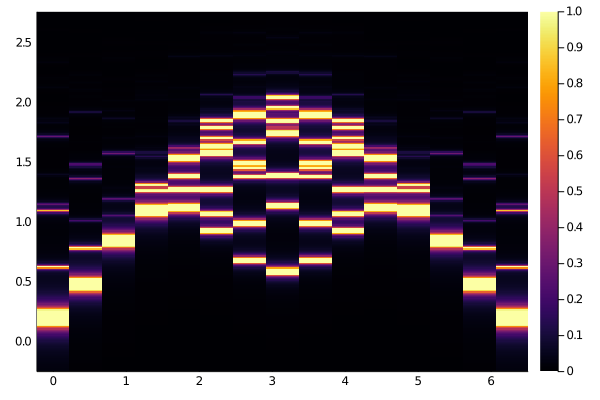
\includegraphics[width=0.45\textwidth]{../figures/fig008.png}
	}
	\\
	\subfloat[$\beta = 0.9$]{
		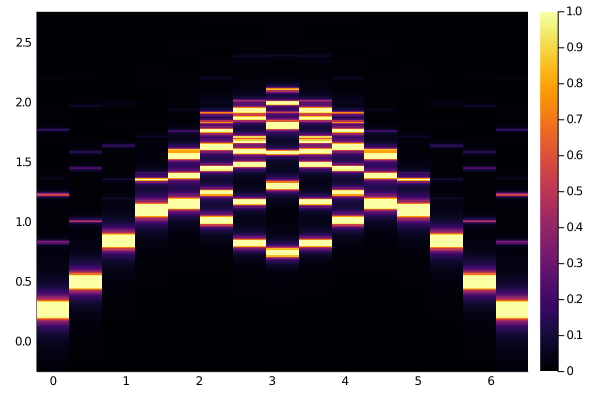
\includegraphics[width=0.45\textwidth]{../figures/fig004.png}
	}
	\subfloat[$\beta = 0.85$]{
		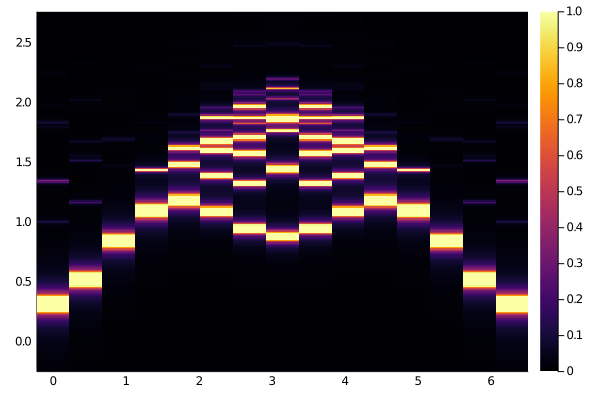
\includegraphics[width=0.45\textwidth]{../figures/fig005.png}
	}
	\\
	\subfloat[$\beta = 0.80$]{
		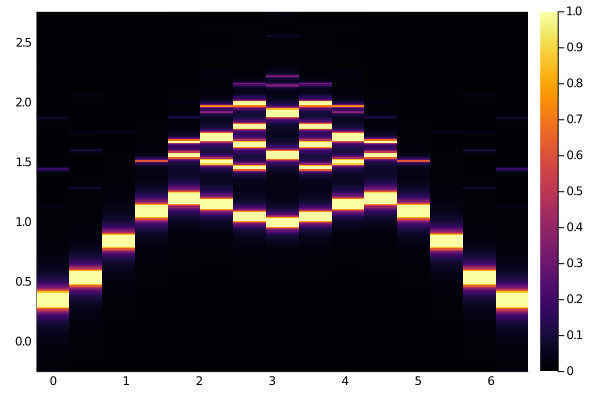
\includegraphics[width=0.45\textwidth]{../figures/fig006.png}
	}
	\subfloat[$\beta = 0.75$]{
		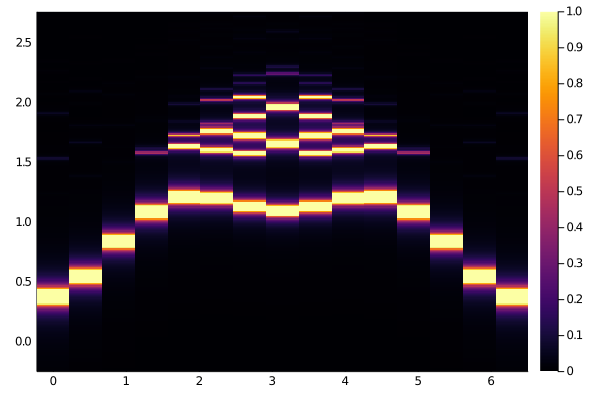
\includegraphics[width=0.45\textwidth]{../figures/fig007.png}
	}
	\\
	\subfloat[$\beta = 0.65$]{
		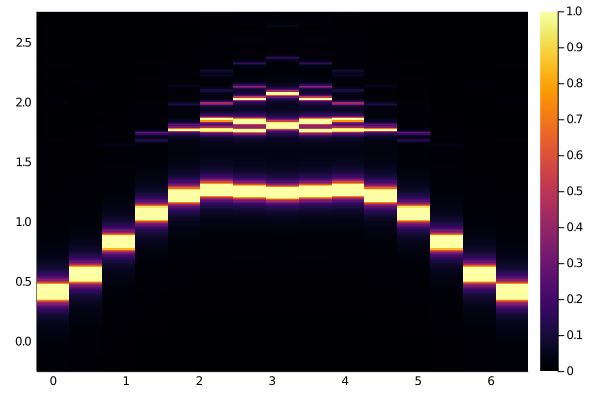
\includegraphics[width=0.45\textwidth]{../figures/fig009.png}
	}
	\subfloat[$\beta = 0.5$]{
		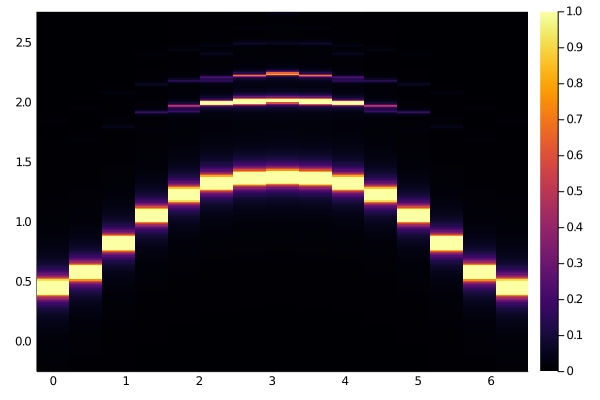
\includegraphics[width=0.45\textwidth]{../figures/fig010.png}
	}
	\caption{Spectral function $S(q,\omega)$ of a single spin flip (magnon excitation) for $\alpha = 0$ and various $\beta$ points.}\label{fig:XY_beta_dep}
\end{figure}
We can observe the continuum being pushed up while the value of $\beta$ decreases. Eventually the gap opens up and we can see a quasiparticle peak. For even higher $\beta$ the continuum is destroyed and the ladder spactrum appears around $k = \pi$. (In order to say more on when the gap opens up and whether the ladder spectrum in not only an artifact of small system size we need to investigate the model for larger lattices.)

\subsection{Anisotropy Effects}
Let us now investigate effects the anisptropy has on the spectral function of a single spin flip in the~XXZ~model. 

\begin{figure}
	\centering
	\subfloat[$\alpha = 0.9$]{
		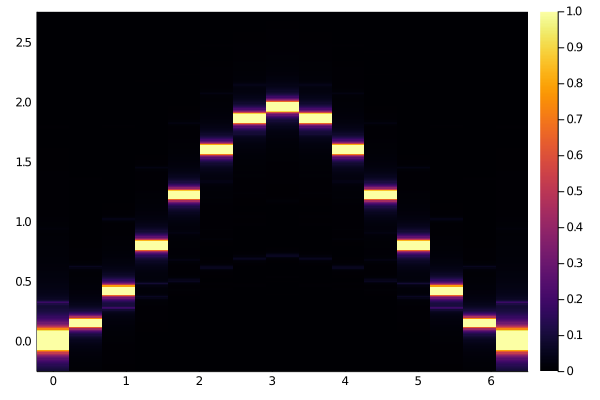
\includegraphics[width=0.45\textwidth]{../figures/fig012.png}
	}
	\subfloat[$\alpha = 0.7$]{
		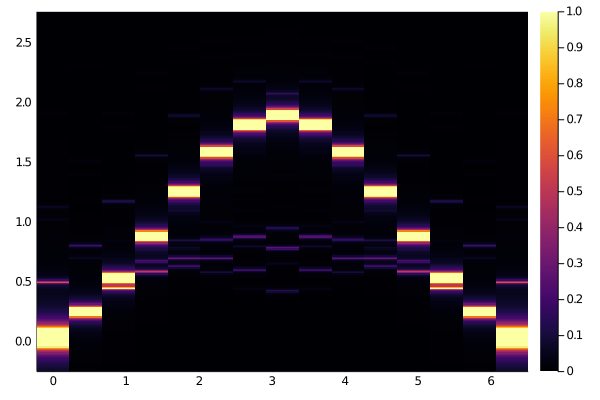
\includegraphics[width=0.45\textwidth]{../figures/fig014.png}
	}
	\\
	\subfloat[$\alpha = 0.6$]{
		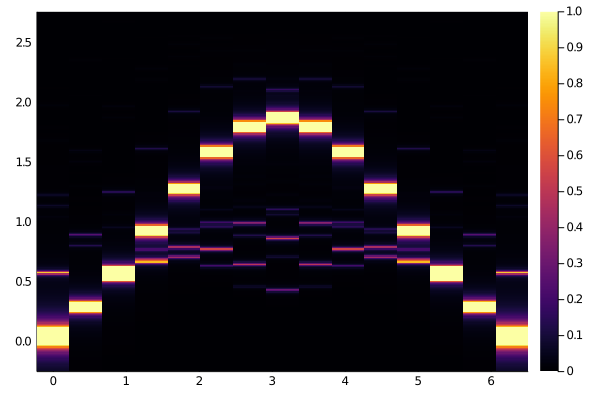
\includegraphics[width=0.45\textwidth]{../figures/fig015.png}
	}
	\subfloat[$\alpha = 0.5$]{
		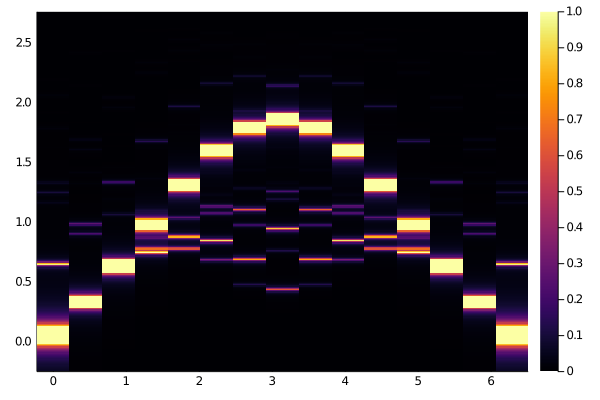
\includegraphics[width=0.45\textwidth]{../figures/fig016.png}
	}
	\\
	\subfloat[$\alpha = 0.4$]{
		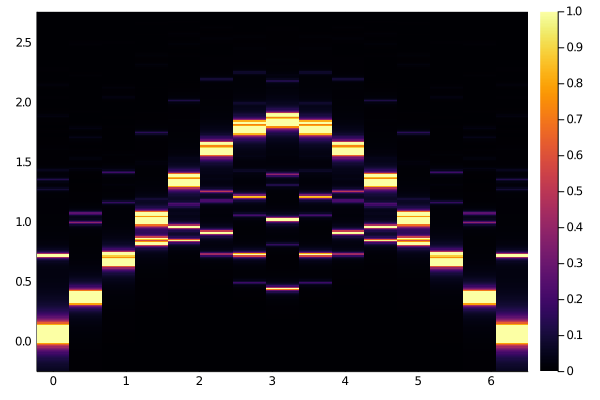
\includegraphics[width=0.45\textwidth]{../figures/fig017.png}
	}
	\subfloat[$\alpha = 0.3$]{
		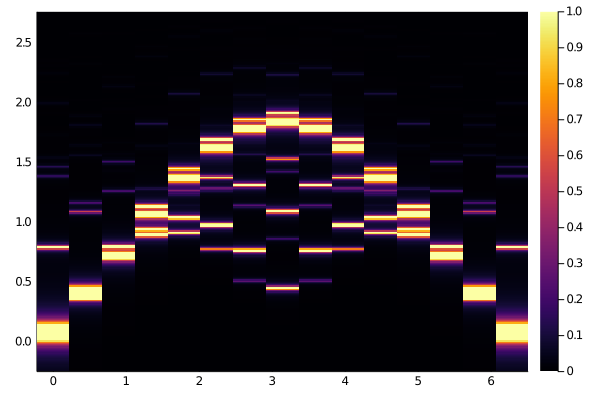
\includegraphics[width=0.45\textwidth]{../figures/fig018.png}
	}
	\\
	\subfloat[$\alpha = 0.2$]{
		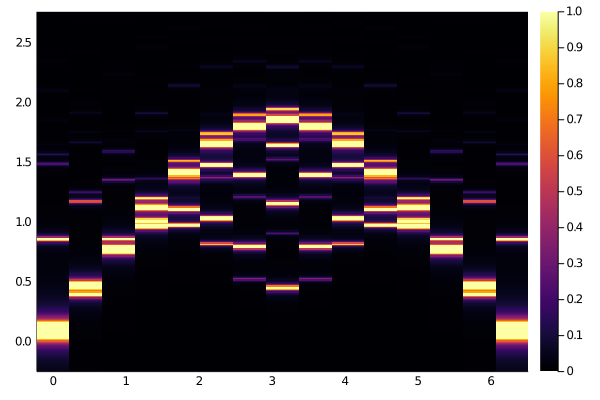
\includegraphics[width=0.45\textwidth]{../figures/fig019.png}
	}
	\subfloat[$\alpha = 0.1$]{
		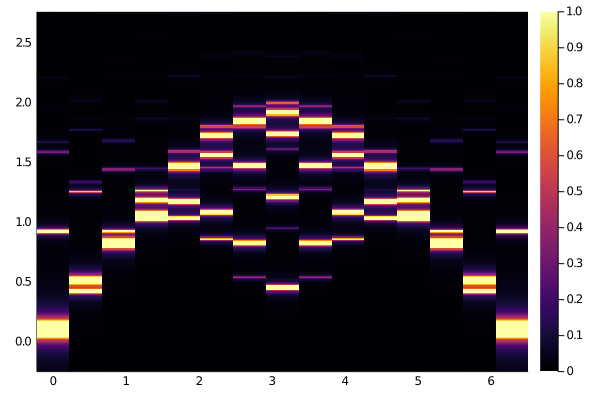
\includegraphics[width=0.45\textwidth]{../figures/fig020.png}
	}
	\caption{Spectral function $S(q,\omega)$ of a single spin flip (magnon excitation) for $\beta = 1$ and various $\alpha$ points.}\label{fig:XXZ_alpha_dep}
\end{figure}

\section{TODO}
\begin{enumerate}
	\item investigate interplay of anisotropy and magnon magnon interactions
\end{enumerate}

\section*{Acknowledgements}
We  kindly  acknowledge  support  by  the  (Polish)  National  Science  Centre  (NCN, Poland)  under  Projects  No. 2016/22/E/ST3/00560 (PW and KW), 2016/23/B/ST3/00839 (KW). The calculations were performed at the ICM cluster.

\bibliographystyle{apsrev4-1}
\bibliography{xxz}

\end{document}
